\documentclass[UTF8,a4paperdui, % draft
]{ctexart}
\usepackage[hidelinks]{hyperref}
\usepackage{bm}
\usepackage{amsmath}
\usepackage{graphicx}
\usepackage{pdfpages}
\usepackage{amsmath}
\usepackage{cite}
\usepackage{caption,subcaption}
\usepackage{geometry}
\usepackage{pdfpages}
\usepackage[ruled,vlined,boxed,linesnumbered]{algorithm2e}
\usepackage{listings}
\usepackage{color}
\lstset {
  basicstyle=\small\ttfamily,
  captionpos=b,
  tabsize=2,
  columns=fixed,
  breaklines=true,
  frame=l,
  numbers=left,
  numberstyle=\small\ttfamily,
  morekeywords= {
    EQUAL, GREATER, LESS, NONE, SOME, abstraction, abstype, and, andalso, array, as, before, bool, case, char, datatype, do, else, end, eqtype, exception, exn, false, fn, fun, functor, handle, if, in, include, infix, infixr, int, let, list, local, nil, nonfix, not, o, of, op, open, option, orelse, overload, print, raise, real, rec, ref, sharing, sig, signature, string, struct, structure, substring, then, true, type, unit, val, vector, where, while, with, withtype, word
  },
  morestring=[b]",
  morecomment=[s]{(*}{*)},
  stringstyle=\color{black},
  identifierstyle=\color{eclipseBlue},
  keywordstyle=\color{red},
  commentstyle=\color{eclipseGreen}
}
\definecolor{eclipseBlue}{RGB}{42,0.0,255}
\definecolor{eclipseGreen}{RGB}{63,127,95}


\geometry{left=4.0cm,right=4.0cm,top=5cm,bottom=5cm}
%%%%%%%%%%%%%%%%%%%%%%%%%%%%
%%%%%%%%%%%%%%%%%%%%%%%%%%%%
\DeclareMathOperator{\net}{net}
\DeclareMathOperator{\sups}{SuperString}
%%%%%%%%%%%%%%%%%%%%%%%%%%%%
%%%%%%%%%%%%%%%%%%%%%%%%%%%%

\makeatletter
\algocf@newcmdside@kobe{LetIn@let}{%
\KwSty{let}%
\ifArgumentEmpty{#1}\relax{ #1}%
\algocf@group{#2}%
\par
}
\algocf@newcmdside@kobe{LetIn@in}{%
\KwSty{in}%
\ifArgumentEmpty{#1}\relax{ #1}%
\algocf@block{#2}{end}{#3}%
\par
}
\newcommand\LetIn[2]{%
\LetIn@let{#1}%
\LetIn@in{#2}%
}
\makeatother

\newcommand\op{\texttt{op}}
\newcommand\ttt{\texttt}
\newcommand\tbf{\textbf}
\newcommand\tit{\textit}
\newcommand\tttt[1]{\text{\ttt{#1}}}
\newcommand\givepar[2]{\ttt{)}$^{#1\ #2}$\ttt{(}}
\usepackage{amssymb}
\usepackage{extarrows}
\begin{document}
\newpage
\newcommand*{\calF}{\mathcal{F}}
\newcommand*{\calH}{\mathcal{H}}
\newcommand*{\vx}{\bm x}
\newcommand*{\vy}{\bm y}
\newcommand*{\vh}{\bm h}
\newcommand{\Figure}[2]{
\begin{figure}[htbp]
\centering
\includegraphics[height=#1]{#2}
\end{figure}
}
%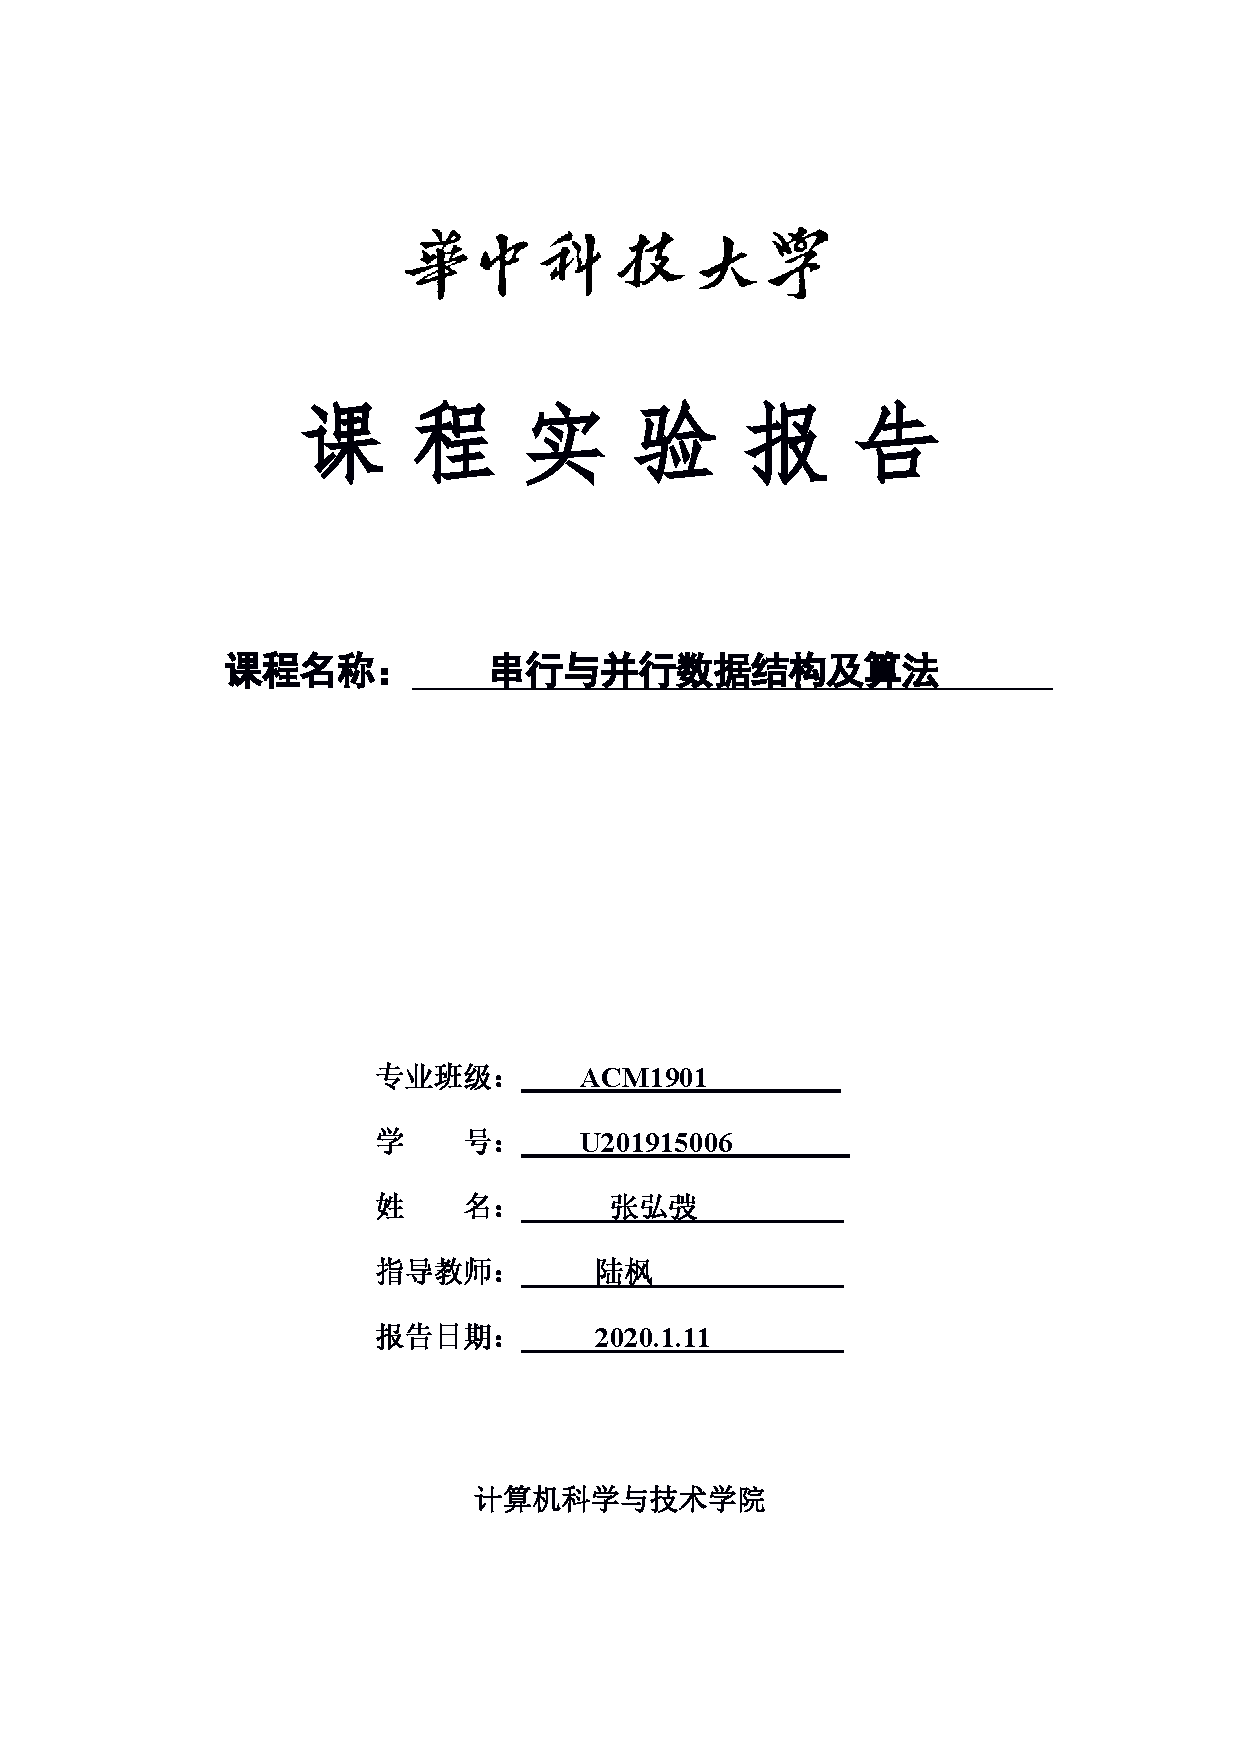
\includepdf{cover}
\tableofcontents
\newpage
\section{无重复排序}
\begin{lstlisting}
val N = getInt();
val A = getIntTable(N);

fun merge([], ys) = ys : int list
  | merge(xs, []) = xs
  | merge(x::xs, y::ys) = 
    if x < y then x::merge(xs, y::ys)
             else y::merge(x::xs, ys);

fun mergesort xs = 
    let fun sort(0, xs) = ([], xs)
          | sort(1, x::xs) = ([x], xs)
          | sort(n, xs) = 
                let val (l1, xs1) = sort((n+1) div 2, xs)
                    val (l2, xs2) = sort(n div 2, xs1)
                in (merge (l1,l2), xs2)
                end 
        val (l, _) = sort (length xs, xs)
    in l end;

val B = mergesort(A);
printIntTable(B);
\end{lstlisting}
\subsection{本关任务}
给出一个具有$N$个互不相同元素的数组,请对它进行升序排序。
\subsection{解法}
我们可以采用归并排序算法解决。
将数据分为
即
\begin{algorithm}
\SetAlgoLined
MergeSort($\langle a_n\rangle$) =\par
\eIf{$|a_n|=1$}{$a_1$}{
\LetIn{
$L\longleftarrow $ MergeSort($\langle a_1,\ a_2,\ \ldots,\ a_{(n+1)/2}\rangle$)\;
$R\longleftarrow $ MergeSort($\langle a_{(n+1)/2},\ \ldots,\ a_{n}\rangle$)\;
}{
Merge($L, R$)}}
\caption{MergeSort}
\end{algorithm}\\
复杂度为
\[
W=O(n\log n)\quad S=O(\log^2n)
\]

\section{最短路}
\subsection{本关任务}
给定一个带权无向图,一个源点,权值在边上。计算从源点到其他各点的最短路径。
\subsection{解法}
可以采用Dijkstra算法解决该问题。

利用二维数组保存两点之间的路径长度,即$A[i][j]$即是编号为$i-1$和$j-1$点之间的路径长度。若无给定长度,则用$\infty$来表示无法两点之间无法到达。创建一个一维数组dis,用以储存源点到每个点的距离。并且集合B为中只有源点a。

(1)在dis数组中寻找一个长度最短的值dis[k],并且保证k点不在集合B中。

(2)再对每个不属于B集合中的点进行长度收缩:如果dis[i]的值dis[k]+A[a][k]的大小,就将dis[i]的值更新为dis[k]+A[a][k]。将k也加入集合B中。

(3)重复上述步骤,直至集合B中有所有点。得到的数组dis的值就是源点到所有对应点的最短路径值。

在SML实际编写程序中,我用99999来替代$\infty$,在比较长度的过程中也方便运算。在最后输出最短路之前,再将所有长度为99999的数据转化成~1说明没有此路径。
\subsection{分析与证明}
Dijkstra算法使用的迭代不超过$n-1$次,在每次迭代的运算中,即比较与更新一共不超过$2(n-1)$次,因此$W=O(n^2)$。每一次的迭代都不能并行运算,但是在每一次的迭代中的比较与收缩长度操作可以同时进行,因此$S=O(n)+1$。
\subsection{样例输入与输出}
样例输入:
\begin{lstlisting}
7 11 5
2 4 2
1 4 3
7 2 2
3 4 3
5 7 5
7 3 3
6 1 1
6 3 4
2 4 3
5 6 3
7 2 1
\end{lstlisting}
样例输出:
\begin{lstlisting}
4 6 7 7 0 3 5 
\end{lstlisting}

\section{最大括号距离}
\subsection{本关任务}
我们定义一个串s是闭合的,当且仅当它由'('和')'构成,而且满足以下条件之一:

空串:这个串为空

连接:这个串由两个闭合的串连接构成

匹配:这个串是一个闭合的串外面包裹一个括号构成的

现在给你一个串,你需要找出所有这个串中匹配的子串(一个闭合的串,并且外侧由括号包裹)中最长的那个,输出它的长度。
\subsection{解法}
现在采用一个stack函数来储存括号的栈。

当栈为空时,判断下一个要入栈的括号的类型:如果是右括号,则必定不会有与之匹配的括号,直接丢弃该右括号;如果时左括号,就将左括号压栈。并在每次栈为空时更新当前最大的匹配括号长度。

当栈不为空时,如果栈顶元素是左括号,即将压栈的括号是右括号,就直接弹出栈顶元素,并增加当前括号距离2。否则将新元素压栈。

由于这种解法只能够解决括号串整体匹配和右括号多于左括号的情况,因此需要将原来的括号串每个元素置换并颠倒,得到新的最大匹配长度不变但括号冗余情况完全相反的括号串。两个串同时经过stack函数的处理,得到的最小的值就是括号匹配的最大的距离。

关键函数stack的代码如下:
\begin{lstlisting}
fun stack([], _, maxpair, tmppair) = Int.max(maxpair, tmppair)
  | stack(x::xs, [], maxpair, tmppair) = 
        if(x=0) 
            then stack(xs, [x], Int.max(maxpair, tmppair), 0)
            else stack(xs, [], Int.max(maxpair, tmppair), 0)
  | stack(x::xs, y::ys, maxpair, tmppair) = 
        if((x=1) andalso (y=0)) 
            then stack(xs, ys, maxpair, tmppair+2)
            else stack(xs, x::y::ys, maxpair, tmppair);
\end{lstlisting}
\subsection{分析与证明}
字符串元素的置换和反转都需要$O(n)$的$W$和$O(1)$、$O(n)$的$S$。

stack函数只需要扫描整个list一遍,因此串行需要的$W$是$O(n)$,$S$也是$O(n)$。
\subsection{样例输入与输出}
样例输入:

50 1 0 1 0 1 1 0 0 1 0 1 1 1 1 0 0 1 0 1 1 1 0 1 0 1 0 1 0 1 1 1 0 1 0 1 1 1 0 1 0 1 1 0 1 1 1 1 0 0 0

样例输出:

6
\section{括号匹配}
\subsection{本关任务}
给定一个括号序列,判断它是否是匹配的。注意( ) ( ) 在本题也当做匹配处理。
\subsection{解法}


\subsection{分析与证明}
\subsection{样例输入与输出}
\section{高精度整数}
\subsection{本关任务}
给定两个任意精度的整数a和b,满足a$\geq$b,求出a+b, a−b, a×b的值。
\subsection{解法}
\subsubsection{加法的计算}
将两个数列进行翻转,即将两个数的最后一位对齐,做相应的加法。

如果两个数相加大于9,就将$c$置为1,在下一位上加上1。
\begin{algorithm}
\SetAlgoLined
$a=(a_1a_2a_3...a_n)_{10}$\par
$b=(b_1b_2b_3...a_m)_{10}$\par
带入该函数时需要将$a$和$b$进行翻转。\par
Addition($a,\ b,\ result,\ c,\ i$) = \par
\eIf{$(a_i\ =\ 0\ andalso\ b_i\ =\ 0)$}{$result_i\ =\ c$}{
\LetIn{
$result_i$ = $a_i$ + $b_i$ + $c$\par
$c$ = ($a_i$ + $b_i$ + $c$) mod 10\par
}{
Addition($a,\ b,\ result,\ c,\ i+1$)}}
\caption{Addition}
\end{algorithm}
\subsubsection{减法的计算}
减法的计算与加法同理,也是将最后一位对齐,从低位开始相减。并用$c$来表示在下一位是否要退位,如果$a-b<0$。
算法如下。
\begin{algorithm}
\SetAlgoLined
$a=(a_1a_2a_3...a_n)_{10}$\par
$b=(b_1b_2b_3...a_m)_{10}$\par
带入该函数时需要将$a$和$b$进行翻转。\par
Subtraction($a,\ b,\ result,\ c,\ i$) = \par
\eIf{$(a_i\ =\ 0\ andalso\ b_i\ =\ 0)$}{$result_i\ =\ c$}{
\LetIn{
\eIf{$a_i-b_i+c\ <\ 0$}{
$c$ = ($a_i$ - $b_i$ + $c$)\par
$result_i\ =\ 10+a_i-b_i+c$
}{$result_i\ =\ a_i-b_i+c$\par
$c\ =\ 0$}
}{
Addition($a,\ b,\ result,\ c,\ i+1$)}}
\caption{subtraction}
\end{algorithm}
\\
\\
\\
\\
\subsubsection{乘法的计算}
先将多位数相乘转换为多个一位数与多位数相乘的乘法。

与上述加法和减法的操作类似,从最末位开始相乘,并用$c$来记录下一位的进位数。

对于第$k$位数完成乘法运算后还要在末尾加上$k-1$个零。

再将所有得到的结果相加。

\begin{lstlisting}
fun onemultiply(a, [], c) = [c]
  | onemultiply(a, b::bs, c) = 
        if (a * b + c> 9) then ((a*b+c)mod 10)::onemultiply(a, bs, (a*b+c) div 10)
                          else (a*b+c)::onemultiply(a, bs, 0);
fun multiply([], bs) = [0]
  | multiply(a::ass, bs) = 
        Add(onemultiply(a, bs, 0), 0::multiply(ass, bs), 0);
\end{lstlisting}


\subsection{分析与证明}
对于加法来说:$n$和$m$相加,需要线性扫描每一个数,因此$W=O(max(|n|,\ |m|)+1)$。对于最优并行算法来说,可以用map操作对对应位数的两个数字相加,并记录每一位需要进位的个数。再将进位数相应相加。重复操作,直到所有每一位的进位数都为0。所有的操作都是并行处理。

在第一次各位数相加时,

因此$S\ =\ O(logn)$。

减法与加法同理,有同样的串行复杂度W。
\subsection{样例输入与输出}
样例输入:

10 2 3 3 3 3 3 3 3 3 3 10 2 3 3 3 3 3 3 3 3 3

样例输出:

4 6 6 6 6 6 6 6 6 6 
0 
5 4 4 4 4 4 4 4 4 2 8 8 8 8 8 8 8 8 9 
\section{素性测试}
\subsection{本关任务}
给定一个数$N$,判断它是否是素数。
\subsection{解法}
利用Miller-Rabin算法来判断数字是否是素数。

费马小定理:当$p$为质数时,有$a^{p-1}\equiv 1(mod\ p)$。

二次探测:如果$p$是一个素数,$0\ < x\ < p$,则方程$x^2\equiv 1(mod\ p)$的解为$x\ =\ 1$或$x\ =\ p\ -\ 1$。

算法流程如下:

输入一个数$x$。

(1)当$x$是偶数或2时可以直接判断。

(2)当$x$是奇数时,组一个比较小的质数$a$,计算$2^s\cdot t\ =\ x\ -\ 1$。

(3)先算出$a^t$,然后进行$s$次平方进行二次探测。即如果在平方的过程中,当前数的平方模$x$与1同余并且该数不等于$1$或$x-1$,那么$x$就是合数,直接退出循环。

(4)根据费马定理判断$a^{p-1}\equiv 1(mod\ p)$是否成立。如果成立,则从第(2)步重新挑选更大的质数$a$再次判断。

\begin{algorithm}
\SetAlgoLined
MergeSort($\langle a_n\rangle$) = \par
\eIf{$|a_n|=1$}{$a_1$}{
\LetIn{
$L\longleftarrow $ MergeSort($\langle a_1,\ a_2,\ \ldots,\ a_{(n+1)/2}\rangle$)\;
$R\longleftarrow $ MergeSort($\langle a_{(n+1)/2},\ \ldots,\ a_{n}\rangle$)\;
}{
Merge($L, R$)}}
\caption{MergeSort}
\end{algorithm}
复杂度为
\[
W=O(n\log n)\quad S=O(\log^2n)
\]

\end{document}
